\documentclass{ximera}
\newcommand{\RR}{\mathbb R}
\renewcommand{\d}{\,d}
\newcommand{\dd}[2][]{\frac{d #1}{d #2}}
\renewcommand{\l}{\ell}
\newcommand{\ddx}{\frac{d}{dx}}
\newcommand{\dfn}{\textbf}
\newcommand{\eval}[1]{\bigg[ #1 \bigg]}


\title{Dig-In: Remainders and the Integral Test}
\author{Jenny Sheldon}


\outcome{Compute the number of terms necessary to estimate a series with given precision using the Integral Test.}
\outcome{Estimate the remainder of an infinite series using the Integral Test.}

\begin{document}
\begin{abstract}
    We investigate how the ideas of the Integral Test apply to remainders.
\end{abstract}
\maketitle


We have split up our infinite sum $S$ into two important pieces: a finite piece $S_n$, which is our estimate, and an infinite piece $R_n$, which is our error or remainder.

\begin{image}
  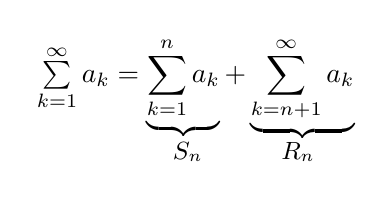
\begin{tikzpicture}
        \node at (0,0) {
           $\sum \limits_{k=1}^\infty a_k  = \underbrace{\sum \limits_{k=1}^n a_k} + \underbrace{\sum \limits_{k=n+1}^\infty a_k} $ 
           };
        \node at (-0.1,-.8) {\small{$S_n$}};
        \node at (1.3, -.8) {\small{$R_n$}};
      \end{tikzpicture}
  \end{image}


We will focus mostly on the remainder, since the estimate is relatively easy to obtain, especially with the use of a computer.  Even though the remainder is an infinite sum, generally we will be concerned with ensuring that the remainder is small -- using whatever definition of ``small'' fits the needs of our problem or situation.

Let's begin with a series $\sum a_k$ and assume that this series converges, and that we would like to estimate its sum.  Let $f(x)$ be the function associated with the sequence ${a_k}$, so that $f(k) = a_k$.  Assume this function $f$ is eventually continuous, positive, and decreasing, so that the Integral Test applies.

Since the Integral Test applies, we know that the integral
\[
\int_N^{\infty} f(x) \, dx
\]
converges to some finite value $L$, but that $L$ is not the sum of the series $\sum a_k$.  While explaining why the Integral Test makes sense, we imagined the terms of our sequence to be a particular Riemann Sum for the integral in question.

\begin{image}
\begin{tikzpicture}
	\begin{axis}[
            domain=0:6,xmin=0,xmax=6,ymin=0,ymax=1.5,
            width=4in,
            height=2in,
            xtick={1,2,...,5},
            ytick={1,.5,.333,.25,.2},
            yticklabels={},%$a_1 = 10$,$a_2=30$,$a_3=90$,$a_4=270$,$a_5=810$},
            axis lines =middle, xlabel={}, ylabel={},
            every axis y label/.style={at=(current axis.above origin),anchor=south},
            every axis x label/.style={at=(current axis.right of origin),anchor=west},
            axis on top,
          ]
          
                    \addplot[color=penColor,fill=penColor,only marks,mark=*] coordinates{(0,1)};  %% closed hole
		\addplot [draw=penColor, fill = fillp] plot coordinates {(0,0) (1,0) (1, 1)(0,1) };   
		
		
          \addplot[color=penColor,fill=penColor,only marks,mark=*] coordinates{(1,1/4)};  %% closed hole
		\addplot [draw=penColor, fill = fillp] plot coordinates {(1,0) (2,0) (2, 1/4) (1,1/4) (1, 0)};          
          
	\addplot[color=penColor,fill=penColor,only marks,mark=*] coordinates{(2,1/9)};  %% closed hole
		\addplot [draw=penColor, fill = fillp] plot coordinates {(2,0) (3,0) (3, 1/9) (2,1/9) (2, 0)};          
          
          \addplot[color=penColor,fill=penColor,only marks,mark=*] coordinates{(3,1/16)};  %% closed hole
          	\addplot [draw=penColor, fill = fillp] plot coordinates {(3,0) (4,0) (4, 1/16) (3,1/16) (3, 0)};          

          
          \addplot[color=penColor,fill=penColor,only marks,mark=*] coordinates{(4,1/25)};  %% closed hole        
          	\addplot [draw=penColor, fill = fillp] plot coordinates {(4,0) (5,0) (5, 1/25) (4,1/25) (4, 0)};          

		  
          \addplot[color=penColor,fill=penColor,only marks,mark=*] coordinates{(5,1/36)};  %% closed hole 
          	\addplot [draw=penColor, fill = fillp] plot coordinates {(5,0) (6,0) (6, 1/36) (5,1/36) (5, 0)};          
           \addplot [draw=penColor,very thick,smooth, domain=.5:6] {1/x^2};
        \end{axis}
\end{tikzpicture}
\end{image}

We can leverage this same picture into helping us estimate the remainder $R_n = \sum_{k=n+1}^\infty a_k$, by imagining that we are trying to add up only those rectangles corresponding to $R_n$.  Remember that we should begin with $a_{n+1}$, or the box whose width is $1$ and whose height is $f(n+1)$.

\begin{image}
\begin{tikzpicture}
	\begin{axis}[
            domain=0:6,xmin=0,xmax=6,ymin=0,ymax=1.5,
            width=4in,
            height=2in,
            xtick={1,2,...,5},
            %ytick={1,.5,.333,.25,.2},
            yticklabels={},
            xticklabels={$n$, $n+1$, $n+2$, $n+3$, $n+4$},%$a_1 = 10$,$a_2=30$,$a_3=90$,$a_4=270$,$a_5=810$},
            axis lines =middle, xlabel={}, ylabel={},
            every axis y label/.style={at=(current axis.above origin),anchor=south},
            every axis x label/.style={at=(current axis.right of origin),anchor=west},
            axis on top,
          ]
          
                  %  \addplot[color=penColor,fill=penColor,only marks,mark=*] coordinates{(0,1)};  %% closed hole
		%\addplot [draw=penColor, fill = fillp] plot coordinates {(0,0) (1,0) (1, 1)(0,1) };   
		
		
          \addplot[color=penColor,fill=penColor,only marks,mark=*] coordinates{(1,1/4)};  %% closed hole
		\addplot [draw=penColor, fill = fillp] plot coordinates {(1,0) (2,0) (2, 1/4) (1,1/4) (1, 0)};          
          
	\addplot[color=penColor,fill=penColor,only marks,mark=*] coordinates{(2,1/9)};  %% closed hole
		\addplot [draw=penColor, fill = fillp] plot coordinates {(2,0) (3,0) (3, 1/9) (2,1/9) (2, 0)};          
          
          \addplot[color=penColor,fill=penColor,only marks,mark=*] coordinates{(3,1/16)};  %% closed hole
          	\addplot [draw=penColor, fill = fillp] plot coordinates {(3,0) (4,0) (4, 1/16) (3,1/16) (3, 0)};          

          
          \addplot[color=penColor,fill=penColor,only marks,mark=*] coordinates{(4,1/25)};  %% closed hole        
          	\addplot [draw=penColor, fill = fillp] plot coordinates {(4,0) (5,0) (5, 1/25) (4,1/25) (4, 0)};          

		  
          \addplot[color=penColor,fill=penColor,only marks,mark=*] coordinates{(5,1/36)};  %% closed hole 
          	\addplot [draw=penColor, fill = fillp] plot coordinates {(5,0) (6,0) (6, 1/36) (5,1/36) (5, 0)};          
           \addplot [draw=penColor,very thick,smooth, domain=.5:6] {1/x^2};
        \end{axis}
\end{tikzpicture}
\end{image}

Notice that all of the rectangles representing the terms of $R_n$ are completely below the graph of $f(x)$.  In symbols,
\[
R_n = \sum_{k=n+1}^\infty a_k < \int_n^\infty f(x) \, dx.
\]
The error is bounded above by the integral.  Assuming we can evaluate the integral, we can give an upper bound for the error $R_n$.

\begin{example}
Consider the series $\sum_{k=1}^\infty \frac{1}{k^2}$.  Give an upper bound for the error involved with using $S_4$ in place of $S$.

\begin{explanation}
The question is asking us to overestimate the value of $R_4$.  Since $f(x) = \frac{1}{x^2}$ is continuous, positive, and decreasing on $[1, \infty)$, let's use the Integral Test to make our overestimate.

We have just seen that
\[
R_4 < \int_{\answer[given]{4}}^{\infty} \frac{1}{x^2}\, dx.
\]

We can evaluate the integral above.
\[
\int_{4}^{\infty} \frac{1}{x^2} = \lim_{b \to \infty} \int_4^b \frac{1}{x^2}\, dx = \lim_{b \to \infty} \left [ \frac{1}{\answer[given]{-1}}x^{\answer[given]{-1}} \right ]_4^{\infty} = \answer[given]{0.25}
\]

Since $R_4$ is less than the value of this integral, we find that $R_4 < \answer[given]{0.25}$.
\end{explanation}


In the event that our application requires us to work with an overestimate for the sum $S$, we can combine our information about $R_n$ with our estimate $S_n$ to get an upper bound for $S$.  In other words, 
\[
S = S_n + R_n < S_n + \int_{n}^{\infty} f(x)\, dx.
\]

\begin{question}
Consider again $\sum_{k=1}^\infty \frac{1}{k^2}$.  Using $n=4$ and the information we found in the previous example, what is an upper bound for the value of this series?
\begin{prompt}
$S < S_n + \int_4^{\infty} \frac{1}{x^2} \, dx = \answer[given]{1 + \frac{1}{4} + \frac{1}{9} + \frac{1}{16}} + \answer[given]{0.25} = \answer[given]{1+\frac{1}{4} + \frac{1}{9} + \frac{1}{16} + 0.25}$
\end{prompt}
\end{question}
\end{example}

Recall that there are two types of questions we can ask about remainders.
\begin{enumerate}
    \item What is the error involved with using a specified number of terms?
    \item How many terms of a series (what is the value of $n$) should we use to obtain a desired precision?
\end{enumerate}
We've covered the first of these questions; let's turn our attention to the second.

\begin{example}
How many terms of the series $\sum_{k=1}^{\infty}\frac{1}{k^2}$ do we need to add in order to guarantee that the estimate $S_n$ is within $0.01$ of the actual sum $S$?

\begin{explanation}
This question is asking us to find a value of $n$ which will guarantee that $S - S_n < 0.01$.  Since the function $f(x) = \frac{1}{x^2}$ is continuous, positive, and decreasing on $[1, \infty)$, let's use the Integral Test to find our answer.

The Integral Test gives us that for any value of $n$, 
\[
R_n < \int_{\answer[given]{n}}^{\infty} \frac{1}{x^2}\, dx = \frac{1}{n}.
\]
Since the remainder is less than the value of the integral, if we make the value of the integral less than $0.01$, then the remainder will also be less than this value.  In symbols, if for a given value of $N$
\[
R_N < \int_N^{\infty} f(x)\, dx < 0.01, 
\]
then
\[
R_N < 0.01
\]
for that same value $N$.  In our case, if we want
\[
R_n < \int_n^{\infty} \frac{1}{x^2}\, dx = \answer[given]{\frac{1}{n}} < 0.01
\]
by solving the second inequality for $n$, we can see that this is true for $n > \answer[given]{100}$.  In other words, if $n > \answer[given]{100}$, then $R_n < 0.01$, as requested.
\end{explanation}
\end{example}

Notice that in the previous example, any larger value of $n$ will also do.  So, as long as we add up at least a hundred terms, the value of $S_n$ will be within $0.01$ of the sum $S$.  Since we know in this case that $\sum_{k=1}^\infty \frac{1}{k^2} = \frac{\pi^2}{6}$, we could check this ourselves!

Finally, it's worth noting that the Integral Test can actually take us quite a bit further than we've gone here.  You might have already noticed that, with the proper setup, the value of the integral can provide an estimate for the entire sum $S$.  Whether this estimate is good enough depends, of course, on your situation.  Furthermore, if we had been clever about how we had organized our rectangles corresponding to the sequence $a_k$ and a Riemann Sum for the integral, we could also come up with a lower bound for the error.  Creating such a lower bound is not as frequently useful as creating an upper bound -- but again, this depends entirely on your application!




\end{document}